\documentclass[journal]{IEEEtran}

% Core packages
\usepackage{cite}
\usepackage{amsmath,amssymb}
\usepackage{graphicx}
\usepackage{booktabs}
\usepackage{multirow}
\usepackage{float}
\usepackage{placeins}
\usepackage{flafter} % a float never appears before its first reference
\usepackage{dblfloatfix}
\usepackage{xcolor}
\usepackage{url}
\usepackage[hidelinks]{hyperref}
\usepackage[T1]{fontenc}
\usepackage[utf8]{inputenc}

\graphicspath{{./images/}}

% Float placement tuning for IEEE two-column layout
\renewcommand{\dbltopfraction}{0.95}
\renewcommand{\topfraction}{0.95}
\renewcommand{\textfraction}{0.05}
\renewcommand{\floatpagefraction}{0.80}
\renewcommand{\dblfloatpagefraction}{0.80}
\setcounter{topnumber}{5}
\setcounter{dbltopnumber}{5}
\setcounter{totalnumber}{8}

\usepackage{etoolbox}

\makeatletter
\patchcmd{\thebibliography}
  {\clubpenalty4000}
  {\clubpenalty4000
   \setlength{\itemsep}{0pt}
   \setlength{\parskip}{0pt}}
  {}{}
\makeatother


\begin{document}
\title{ADMET-Bench: Task-Dependent Performance of GNNs and Pretrained Models in ADMET Prediction}

\author{
\IEEEauthorblockN{
Martin Stamenov\IEEEauthorrefmark{1},
Mila Gjurovska\IEEEauthorrefmark{1},
Viktorija Vodilovska\IEEEauthorrefmark{2} and
Ilinka Ivanoska\IEEEauthorrefmark{1}
}

\IEEEauthorblockA{\IEEEauthorrefmark{1} %1st affiliation
Faculty of Computer Science and Engineering, Ss Cyril and Methodius University, Skopje, N. Macedonia}

\IEEEauthorblockA{\IEEEauthorrefmark{2} %2nd affiliation
Graduate School of Life Sciences, Utrecht University, Utrecht, The Netherlands}

martin.stamenov@students.finki.ukim.mk, mila.gjurovska@students.finki.ukim.mk, v.vodilovska@students.uu.nl, ilinka.ivanoska@finki.ukim.mk

\thanks{Ilinka Ivanoska is the corresponding author.}
\thanks{Martin Stamenov and Mila Gjurovska contributed equally.}
\thanks{Supported by Faculty of Computer Science and Engineering, Skopje, N. Macedonia.}
}

\maketitle

\begin{abstract}
The reliability of structure-based prediction of absorption, distribution, metabolism, excretion, and toxicity (ADMET) properties varies substantially across endpoints, yet many studies compare molecular models without matched tuning or leakage controls. This work benchmarks graph neural networks (GNNs), frozen pretrained molecular representations (ChemBERTa, MolCLR), and fingerprint baselines across six Therapeutics Data Commons endpoints---four pharmacokinetic regression tasks and two toxicity classification tasks---under scaffold-split evaluation. To make the comparison fair, every model family receives a matched 50-trial, validation-selected tuning budget and is evaluated as the median over ten seeds; architecture, hyperparameter, and decision-threshold selection use validation data only, and the held-out test split is used exclusively for final performance estimation, never for any selection. Under this leakage-controlled, budget-matched protocol, \emph{no model family dominates}: differences between families fall within the seed-to-seed range on most endpoints. The GNN is clearly best only on Caco-2 permeability (R$^2 \approx 0.48$), and a controlled ablation shows this advantage comes entirely from auxiliary physicochemical descriptors rather than the graph representation; simple Morgan fingerprints are competitive on hERG (AUC $\approx 0.77$) and give the best median on both clearance endpoints, and MolCLR is best on Tox21. For hepatocyte clearance and half-life, all models yield near-zero or negative R$^2$. Across the six datasets, no hyperparameter-optimization metaheuristic consistently outperforms random search at a 50-trial budget. We further show that common shortcuts---selecting the optimizer on the test set, and reporting single best-trial runs---can substantially inflate a favored model's apparent advantage. ADMET model selection is therefore endpoint-specific, and fair, leakage-controlled, seed-averaged evaluation is essential for realistic assessment of molecular machine-learning models.
\end{abstract}

\begin{IEEEkeywords}
graph neural networks, ADMET prediction, molecular property prediction, scaffold-split, pretrained models, drug discovery, benchmarking
\end{IEEEkeywords}


\section{Introduction}
\label{sec:intro}

\IEEEPARstart{P}{redicting} molecular ADMET (Absorption, Distribution, Metabolism, Excretion, and Toxicity) properties is a central task in computational drug discovery, enabling early identification of promising candidates and flagging safety liabilities before costly synthesis and \emph{in vivo} testing~\cite{zhang2025admet}. Graph Neural Networks (GNNs) have become prominent in this domain by treating molecules as graphs in which atoms serve as nodes and bonds as edges, enabling task-specific learning through message passing that encodes both local chemical motifs and global topological patterns inaccessible to fixed-length descriptors~\cite{gilmer2017neural, yang2019dmpnn, attentiveFP}.

Beyond GNNs, a diverse range of approaches has been applied to ADMET prediction. Pretrained molecular encoders such as ChemBERTa~\cite{chemberta2} and MolCLR~\cite{molclr} leverage self-supervised learning on large molecular corpora to produce reusable representations. Classical fingerprint-based methods, including Morgan (ECFP) fingerprints~\cite{rogers2010ecfp} paired with traditional ML or MLP predictors, remain competitive baselines~\cite{maplight, rdkit2d_mlp}. Although these approaches differ in architecture and encoding strategy, all model families evaluated here rely exclusively on molecular structure as input, representing the same underlying 2D molecular graph or SMILES string~\cite{weininger1988smiles} through different feature representations. Across these paradigms, strong predictive performance has been reported, often achieving state-of-the-art results on individual tasks~\cite{huang2021therapeuticsdatacommonsmachine}.

Despite this progress, model selection in practice remains unclear. Different models perform inconsistently across tasks, and most published studies optimize performance for individual architectures or compare methods under different splits and experimental conditions, making direct comparison unreliable~\cite{wu2018moleculenet, yang2019dmpnn}. Crucially, many works rely on random data splits, which allow structurally similar molecules to appear in both training and test sets, producing overly optimistic estimates that do not reflect the real-world scenario of predicting properties for new chemical scaffolds. As a result, practitioners still lack consistent guidance on model selection, endpoint-specific reliability, and the conditions under which molecular structure alone provides sufficient predictive information~\cite{wu2018moleculenet, huang2021therapeuticsdatacommonsmachine}.

Scaffold-based splitting~\cite{doi:10.1021/jm9602928} partitions compounds by core ring structures and serves as a realistic evaluation protocol reflecting prospective drug discovery, where models must generalize to novel chemical series. In this work, we investigate how predictive performance depends on the underlying task and evaluation protocol, with a focus on identifying when molecular structure alone provides sufficient signal. This issue is particularly important for pharmacokinetic endpoints such as clearance and half-life, where inaccurate predictions can affect compound prioritization. Models that appear accurate under weak evaluation protocols may provide misleading support for early-stage screening decisions.

Benchmarking should therefore identify not only which model performs best, but also which endpoints are predictable from molecular structure under realistic scaffold-shift conditions. This motivates endpoint-specific model selection, where the modeling approach is chosen according to the biological and experimental characteristics of the endpoint. From a biomedical informatics perspective, ADMET predictors act as decision-support components in early-stage drug-discovery pipelines. If such models are evaluated under overly optimistic protocols, they may produce overconfident predictions for novel scaffolds and misguide prioritization. Understanding endpoint-specific reliability under scaffold shift is therefore essential for trustworthy AI in translational drug-discovery workflows.

The main contributions of this study are as follows:
\begin{itemize}
 \item A systematic benchmark of graph-based, fingerprint-based, and pretrained molecular representation models across six ADMET endpoints from the TDC benchmark.
 \item Evaluation under scaffold-split conditions, enabling realistic assessment of generalization to structurally distinct compounds.
 \item Analysis of model behavior across endpoints with different biological characteristics, showing how predictive performance varies between permeability, toxicity, clearance, and half-life tasks.
 \item Assessment of seven hyperparameter-optimization strategies for the GNN across six ADMET endpoints under a common 50-trial budget, kept separate from the matched-budget model-family comparison.
 \item Identification of endpoint-specific cases where molecular structure provides sufficient predictive signal, and cases where structure-only representations remain limited, motivating biological or assay-level information in future ADMET models.
\end{itemize}

The remainder of this paper is organized as follows. Section~II reviews related work. Section~III describes materials and methods. Section~IV presents experimental results. Section~V discusses implications and limitations. Section~VI concludes.

\section{Related Work}
\label{sec:related}

\subsection{ADMET Prediction}

The TDC ADMET benchmark~\cite{huang2021therapeuticsdatacommonsmachine} has become the standard evaluation platform for molecular property prediction. Representative molecular-property prediction approaches include fingerprint-based methods such as MapLight and RDKit2D+MLP, graph neural networks including GCN, GIN, D-MPNN and AttentiveFP, and pretrained molecular representation models such as MolCLR and ChemBERTa. These approaches span fixed descriptors, task-specific graph learning, and self-supervised molecular representation learning.

The TDC leaderboards~\cite{tdc_admet_leaderboard} reveal that several top-performing approaches rely on comparatively simple architectures. MapLight~\cite{maplight} uses random forests and SVMs on node embeddings, while RDKit2D+MLP~\cite{rdkit2d_mlp} passes 200 physicochemical descriptors through a standard MLP. On certain datasets, even Random Forest or XGBoost achieves top results, motivating ensemble approaches such as FCA~\cite{cfa}.

Among GNN-based methods, AttentiveFP~\cite{attentiveFP} employs GCN/GAT layers with GRU-based attention readout, achieving top-5 results on many TDC datasets. Standard architectures appearing prominently in molecular benchmarks include GCN~\cite{kipf2017gcn}, GIN~\cite{xu2019gin}, and D-MPNN~\cite{yang2019dmpnn}, which operates on bond-level rather than atom-level messages.

Self-supervised pretraining has been adapted from NLP to molecular graphs via two main paradigms: attribute masking~\cite{attrMasking}, which reconstructs removed node or edge features, and contrastive learning~\cite{contrativeLearning}, which trains encoders to produce similar embeddings for augmented views of the same molecule. MolCLR~\cite{molclr} extends contrastive learning with three graph augmentation strategies (atom masking, bond deletion, subgraph removal), demonstrating improved downstream ADMET prediction. These techniques underpin most pretrained molecular representation models, which follow a common paradigm: self-supervised pretraining on large unlabeled corpora, optional multi-task supervised training, and task-specific fine-tuning. Representative examples include DeepMol~\cite{deepMol} and MolE~\cite{molE}. ChemBERTa~\cite{chemberta2} applies a RoBERTa transformer to SMILES strings pretrained on 77M molecules from ZINC-15~\cite{sterling2015zinc15}, while MolBERT~\cite{molbert} combines SMILES masked language modeling with auxiliary physicochemical objectives. A practical concern with pretrained models is their large parameter count. MiniMol~\cite{miniMol} addresses this using MPNN++ ($\sim$10M parameters) to achieve competitive TDC performance at lower computational cost.

\paragraph{Scaffold Split Challenges}
Transformer-based models frequently show severe generalization drops under scaffold splitting, with strong validation scores that collapse toward chance-level performance on held-out scaffolds~\cite{yang2019dmpnn,chemberta2}. Wu et al.~\cite{wu2018moleculenet} introduced MoleculeNet with scaffold-splitting to reflect prospective drug discovery generalization; we revisit this collapse in Section~\ref{sec:results}.

\subsection{Hyperparameter Optimization for Molecular ML}

HPO is a key performance driver in molecular ML, where small, noisy datasets amplify sensitivity to hyperparameter configuration. Bergstra and Bengio~\cite{bergstra2012random} established Random Search as a strong baseline, showing it outperforms grid search when only a subset of hyperparameters is influential. Bayesian methods such as TPE~\cite{bergstra2011tpe}, implemented in Optuna~\cite{akiba2019optuna}, improve sample efficiency by modeling the hyperparameter-performance relationship. Population-based metaheuristics, including PSO~\cite{kennedy1995pso}, GA~\cite{holland1975ga}, and ABC~\cite{karaboga2005abc}, provide broader exploration but may require larger budgets to converge. SA~\cite{saopt} offers a middle ground by accepting suboptimal moves early to escape local optima. Despite their widespread use in combinatorial optimization, systematic comparisons of these HPO strategies for molecular property prediction remain scarce, particularly under scaffold-split protocols, motivating our evaluation within a unified ADMET benchmark.

\subsection{Challenges in Molecular ML}

ADMET prediction remains challenging because many endpoints exhibit distribution shifts under scaffold splitting, limited dataset sizes, and class imbalance. These factors can substantially affect model rankings and generalization estimates, motivating the use of multi-seed evaluation and confidence-interval-based reporting throughout this study.


\section{Materials and Methods}
\label{sec:methods}

\subsection{Framework Overview}
\label{sec:framework}

To compare model families under realistic generalization conditions, we use a benchmarking framework (Fig.~\ref{fig:benchmark-framework}) that applies the same scaffold partitions, datasets, and metrics across the GNN and the frozen-pretrained/fingerprint pipelines. The framework coordinates dataset loading, scaffold-split partitioning, training, metric computation, multi-seed analysis, and HPO comparison against Random Search. Fixing splits and metrics across models reduces experimental confounds and enables direct comparison between model families~\cite{wu2018moleculenet}.

\begin{figure}[!t]
 \centering
 \includegraphics[width=\columnwidth,height=0.58\textheight,keepaspectratio]{architecture.png}
 \caption{Modular benchmarking architecture for evaluating molecular graph neural networks and pretrained models on ADME and toxicity prediction tasks. The framework consists of three layers: a benchmark orchestration layer coordinating datasets and experimental configurations, a model execution layer evaluating multiple neural architectures, and an evaluation pipeline.}
 \label{fig:benchmark-framework}
\end{figure}

\subsection{Datasets and Evaluation Protocol}
\label{sec:datasets}

We evaluate all models on six molecular property prediction tasks drawn from the TDC ADMET benchmark~\cite{huang2021therapeuticsdatacommonsmachine}, covering four pharmacokinetic (ADME) regression tasks and two toxicity classification tasks. This protocol reflects practical drug discovery scenarios, where models must generalize to novel chemical series. Fig.~\ref{fig:class-distribution} provides an overview of data provenance and class composition across all six datasets.

\subsubsection{ADME Regression Tasks}

\paragraph{Caco-2 Permeability (Caco2\_Wang)}
The dataset contains 910 compounds with permeability values reported in log(cm/s) units and is commonly used as an \emph{in vitro} surrogate of intestinal absorption~\cite{artursson1991caco2}.

\paragraph{Half-Life Prediction (Half\_Life\_Obach)}
The dataset contains 667 compounds with plasma half-life measurements. Target values are log-transformed prior to standardization to reduce skewness.

\begin{figure*}[!t]
 \centering
 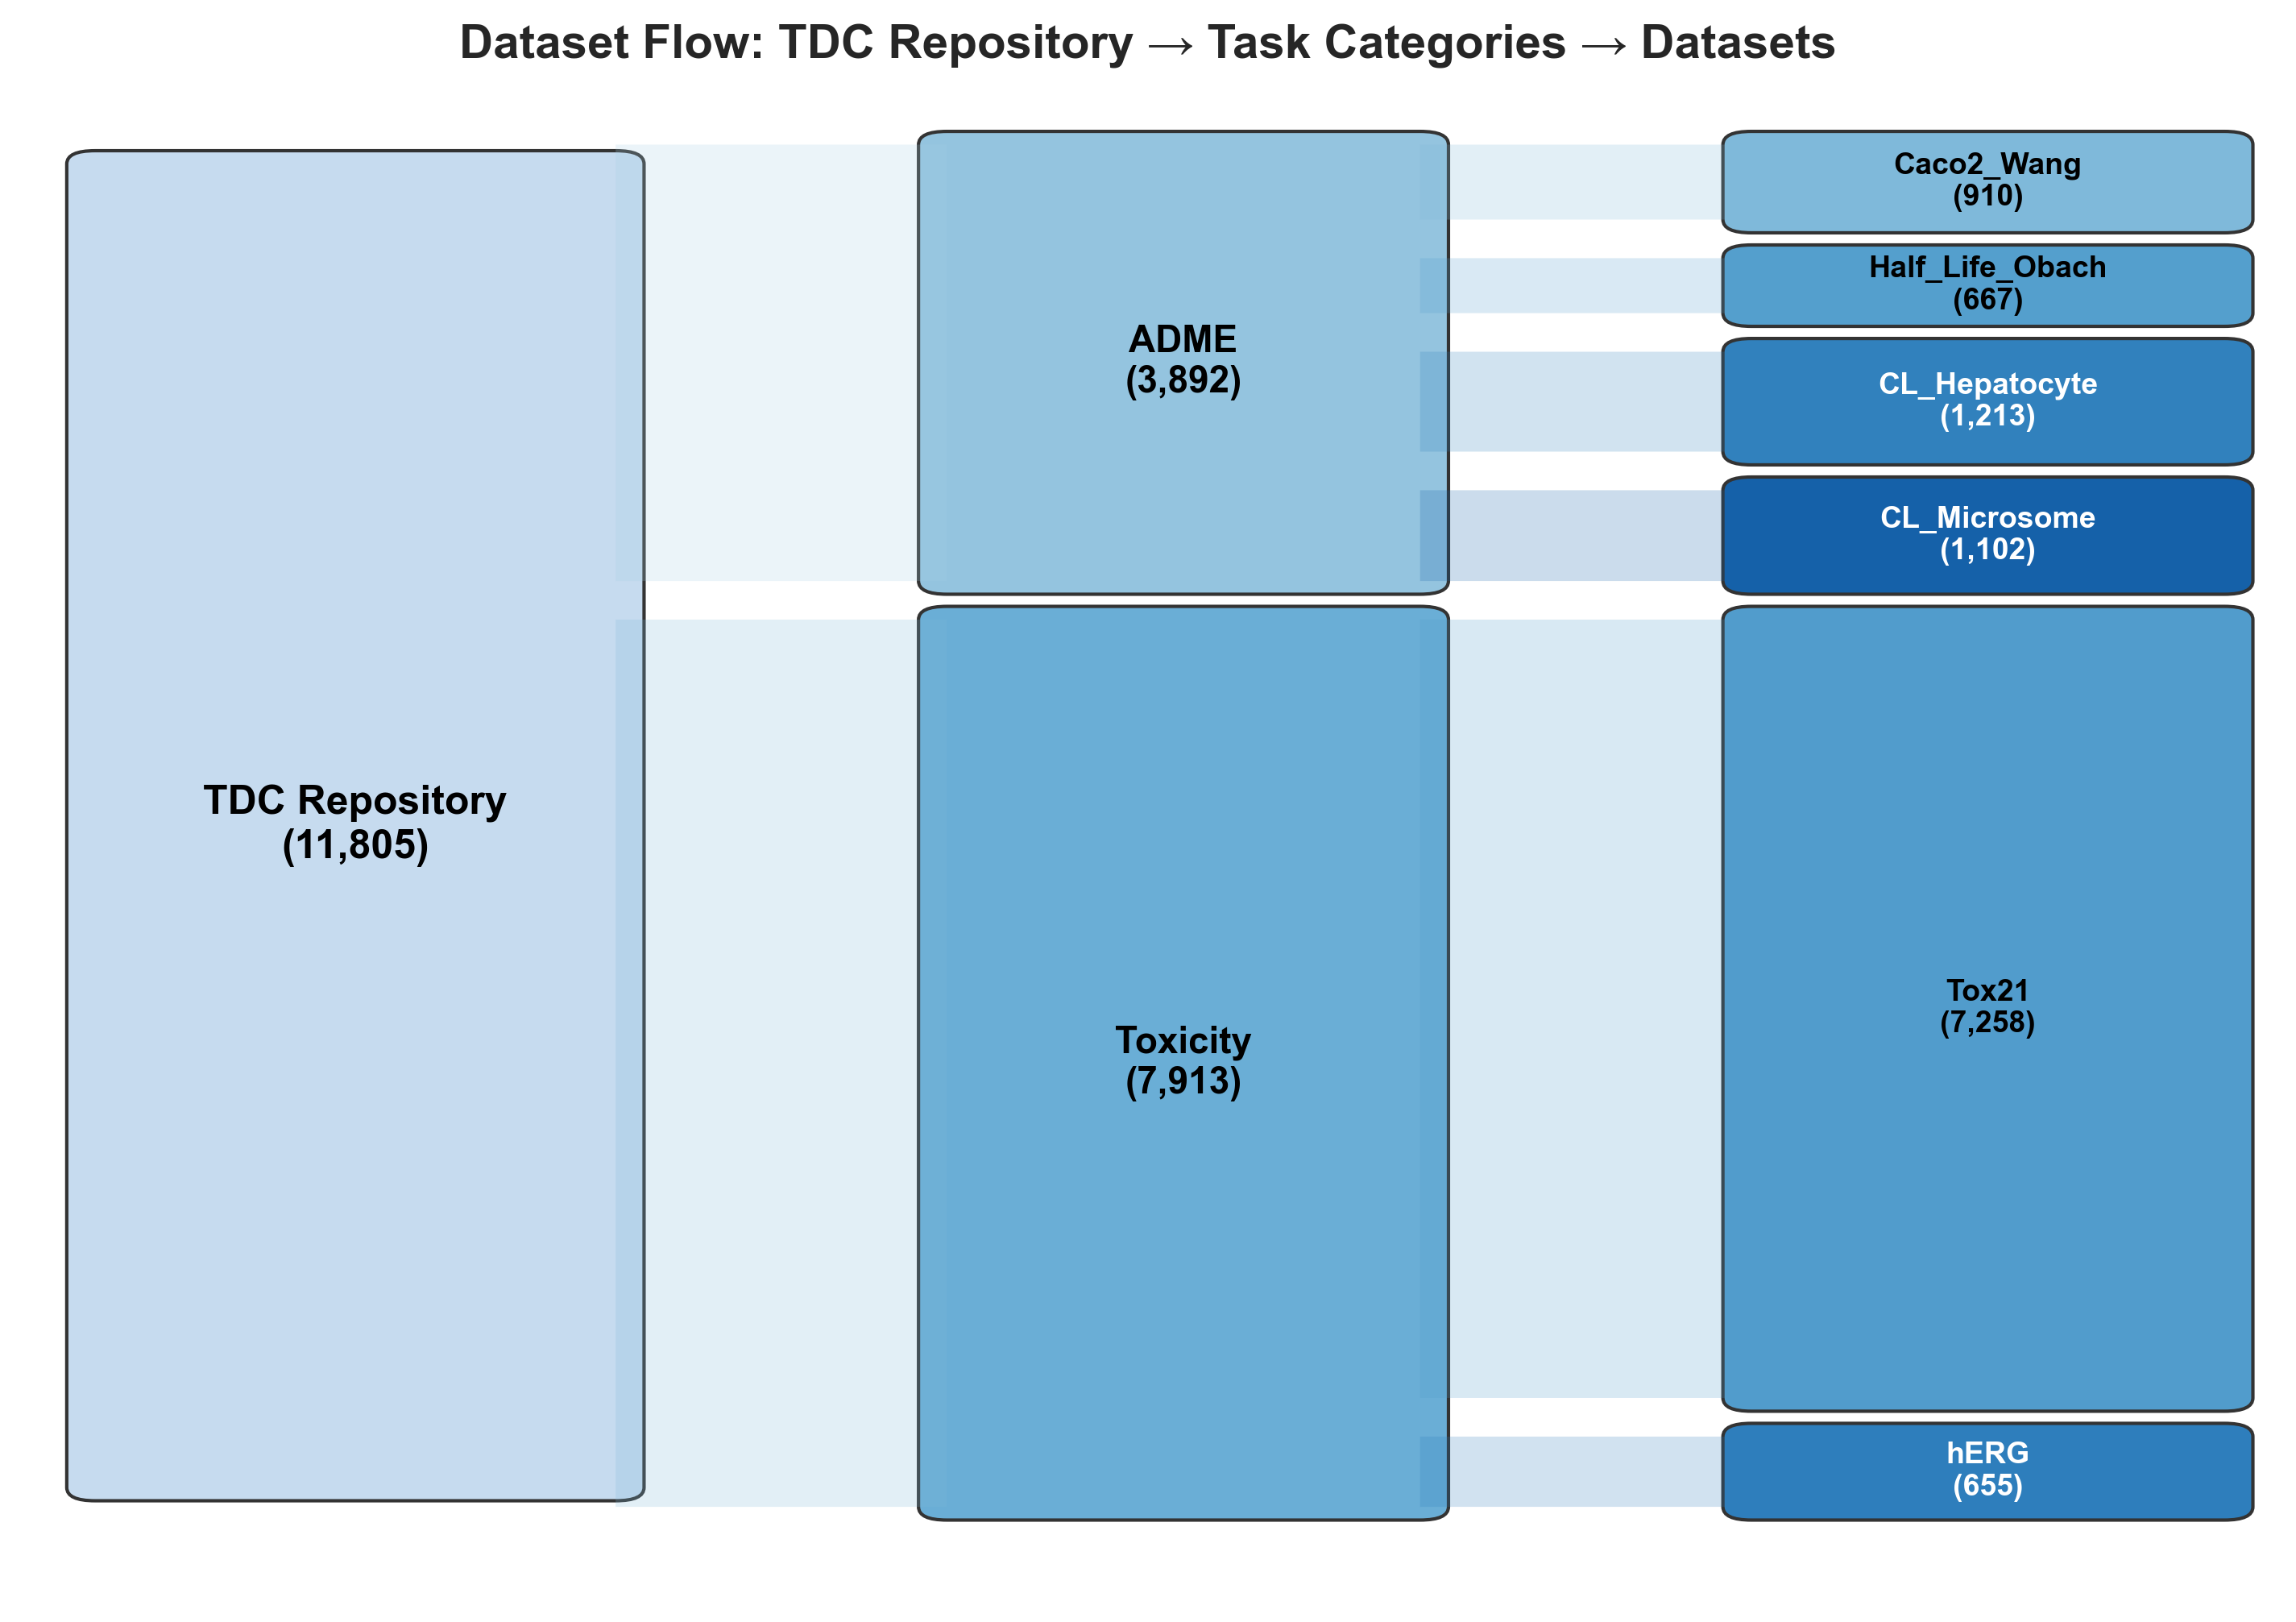
\includegraphics[width=0.75\textwidth,height=0.42\textheight,keepaspectratio]{sankey-diagram.png}
 \caption{Overview of data source and task labels. This flowchart details the $11{,}805$ total instances catalogued in the TDC Repository. After removing molecules with invalid SMILES or failed graph conversion, $10{,}627$ molecules are retained for training and evaluation.}
 \label{fig:class-distribution}
\end{figure*}

\paragraph{Hepatocyte Clearance (Clearance\_Hepatocyte\_AZ)}
The AstraZeneca dataset contains 1,213 compounds with intrinsic clearance measurements obtained from human hepatocyte assays~\cite{huang2021therapeuticsdatacommonsmachine}.

\paragraph{Microsomal Clearance (Clearance\_Microsome\_AZ)}
The AstraZeneca microsomal clearance dataset contains 1,102 compounds with human liver microsome measurements. Targets are log-transformed and standardized using training-set statistics.

\subsubsection{Toxicity Classification Tasks}

\paragraph{Tox21 Nuclear Receptor: Androgen Receptor (Tox21 NR-AR)}
The dataset contains 7,258 compounds with binary androgen receptor activity labels and exhibits substantial class imbalance, with approximately 4.2\% positive samples in the full corpus (rising to $\approx$4.9\% on the scaffold-split test set, see Section~\ref{sec:results}).

\paragraph{hERG Cardiotoxicity (hERG)}
The hERG dataset contains 655 compounds with blocker/non-blocker labels and is widely used for cardiotoxicity assessment~\cite{sanguinetti2006herg}.

\paragraph{Splitting and evaluation protocol}
We use the TDC scaffold-split function, which partitions compounds by Bemis-Murcko scaffolds~\cite{doi:10.1021/jm9602928} so that molecules with structurally distinct core rings appear in different folds. This approximates prospective deployment conditions, where a model must generalize to structurally distinct compound families not seen during training. We further subdivide the scaffold-held training partition into training and validation at the \emph{molecule} level: observations are grouped by canonical SMILES, and each unique molecule---with all of its measurements---is assigned to either training or validation using a fixed random seed (42), so that no molecule can occur in both partitions. A fixed fraction (10\%) of the unique molecules forms the validation set, used for early stopping and model selection; the held-out scaffold test set is left unchanged. The final split proportions are approximately 70/8/22 (train/validation/test) across all datasets.

During HPO, the test split remains \emph{fully held out}, model selection is performed solely on the validation metric. Final performance is reported once on the test split after HPO is complete, preventing any implicit information leakage from repeated test-set evaluations.

\paragraph{Target transformations}
For Half-Life, Hepatocyte, and Microsomal Clearance, targets are log-transformed using $y'=\log(\max(y,\epsilon))$, $\epsilon=10^{-3}$, followed by training-set z-score normalization. Caco-2 targets require only normalization, while classification labels remain binary.

\subsection{Model Families}
\label{sec:model_families}

We evaluate three distinct model paradigms under the same scaffold splits and evaluation metrics, allowing us to assess whether task-specific learning provides advantages over frozen pretrained representations and fixed fingerprint baselines.

\paragraph{GNN models}
We employ graph neural networks trained end-to-end on each task. The GNN backbone is based on stacked GraphConv layers~\cite{morris2019wlgnn} with batch normalization, ReLU activation, and additive residual connections, selected through a preliminary architecture comparison across eight GNN variants (Section~\ref{sec:arch_selection}). Each molecule is represented as a molecular graph constructed from SMILES using RDKit. Atom features include standard atom-level chemical descriptors (8 features); no bond features are used. The GNN encoder produces node embeddings aggregated into a graph-level representation using concatenated global mean and max pooling. Before the prediction head, this pooled representation is concatenated with a small vector of structure-derived physicochemical descriptors computed with RDKit (15 for the ADME/toxicity tasks, e.g.\ molecular weight, cLogP, TPSA, hydrogen-bond donors/acceptors, and Lipinski flags; a 7-descriptor subset for Caco-2). These descriptors carry no biological or assay information and are provided only to the GNN, not to the pretrained or fingerprint baselines. The combined representation is passed to an MLP prediction head with batch normalization and optional dropout; for the small Caco-2 dataset the GNN additionally applies dropout ($0.5$) and Gaussian target-label noise ($\sigma=0.05$). GNN models undergo full hyperparameter optimization (Section~\ref{sec:model_training}).

\paragraph{Pretrained models}
We evaluate two pretrained molecular encoders representing the two major pretrained paradigms: ChemBERTa~\cite{chemberta2} (SMILES-based transformer) and MolCLR~\cite{molclr} (graph-based contrastive model), as representative rather than exhaustive examples. For pretrained encoders, we use a frozen encoder and trainable MLP head setting: embeddings are extracted once per molecule, and an MLP is trained on the train split with early stopping based on the validation split. This frozen-encoder protocol isolates the quality of pretrained representations from downstream optimization effects.

\paragraph{Fingerprint baselines}
We evaluate two fingerprint-based approaches: (i) Morgan fingerprints (ECFP)~\cite{rogers2010ecfp} with an MLP predictor, and (ii) MolE-style learned fingerprints (MolE-FP) with an MLP predictor. The MolE-FP baseline is implemented as Morgan fingerprints followed by a learned projection inspired by the MolE approach~\cite{molE}, rather than the original pretrained MolE encoder. All baselines use the same dataset splits and evaluation metrics as the GNN experiments.

\subsection{Model Training and Configuration}
\label{sec:model_training}

\paragraph{GNN Training}
All GNN models were trained using the Adam optimizer with a batch size of 32. During HPO, models were trained for a maximum of 50 epochs per trial with early stopping (patience = 12). Regression models used mean squared error (MSE) loss, while classification models used binary cross-entropy (BCE) loss with logits. Gradient clipping was applied with a maximum norm of 1.0. The hyperparameter search space is defined in Supplementary Materials (Table S4).

\paragraph{Optimization algorithms}
We evaluate seven HPO strategies: Random Search~\cite{bergstra2012random}, Particle Swarm Optimization (PSO)~\cite{kennedy1995pso}, Artificial Bee Colony (ABC)~\cite{karaboga2005abc}, Genetic Algorithm (GA)~\cite{holland1975ga}, Simulated Annealing (SA)~\cite{saopt}, Hill Climbing (HC)~\cite{russell2010aima}, and Tree-structured Parzen Estimator (TPE)~\cite{akiba2019optuna}. Population-based methods use population size 16. SA uses $T_0=1.0$ with exponential cooling ($\alpha=0.99$), while TPE uses Optuna defaults with median pruning. Search spaces are provided in Supplementary Table S4. Each algorithm is allocated 50 trials per dataset, giving 2{,}100 GNN training runs from the optimizer comparison alone (seven optimizers $\times$ six datasets $\times$ 50 trials). In addition, the study includes a preliminary architecture-selection screen (reported in the Supplementary Material) and 60 multi-seed validation runs for the final selected models. We keep two questions separate. For the \emph{fair model-family comparison} (Table~\ref{tab:model_comparison}), the GNN is tuned with a single predefined optimizer---Random Search---whose configuration is selected on validation and evaluated once on test, matching the 50-trial validation-based budget given to every baseline; the test set is never used to choose the optimizer. The seven-optimizer study is a \emph{separate} analysis of whether optimizer choice affects the GNN, and its outcomes do not feed the model-family comparison.

\begin{table}[!t]
\centering
\caption{Dataset statistics and evaluation metrics (TDC ADMET). ``TDC'' shows compounds catalogued and ``Used'' shows those retained after filtering. RMSE is the primary per-dataset regression metric, the scale-invariant R$^2$ is additionally used for cross-model comparison in Table~\ref{tab:model_comparison}.}
\label{tab:dataset_stats}
\small
\begin{tabular}{lccccc}
\toprule
\textbf{Dataset} & \textbf{Type} & \textbf{TDC} & \textbf{Used} & \textbf{Split} & \textbf{Metric} \\
\midrule
Caco2\_Wang & Regr. & 910 & 819 & Scaffold & RMSE \\
Half\_Life & Regr. & 667 & 601 & Scaffold & RMSE \\
Clear.\_Hep. & Regr. & 1,213 & 1,092 & Scaffold & RMSE \\
Clear.\_Mic. & Regr. & 1,102 & 992 & Scaffold & RMSE \\
Tox21 (NR-AR) & Class. & 7,258 & 6,533 & Scaffold & AUC \\
hERG & Class. & 655 & 590 & Scaffold & AUC \\
\bottomrule
\end{tabular}
\end{table}

\subsection{Experimental Setup}
\label{sec:experimental_setup}

\paragraph{Datasets}
Table~\ref{tab:dataset_stats} summarizes the dataset characteristics across all six tasks.

\paragraph{Evaluation metrics}
Model performance is assessed using RMSE, R$^2$, and MAE for ADME regression tasks, and AUC-ROC and F1-score for toxicity classification tasks. AUC-ROC is the primary ranking metric for classification and is the classification metric used in the paired optimizer comparison (Supplementary Table~S3); F1 is reported in addition because it is more sensitive to the minority class under strong class imbalance.

\paragraph{Multi-seed validation}
To quantify robustness, we retrain the best HPO-selected configuration per dataset across ten seeds $[42, 123, 456, 789, 1011, 2022, 3033, 7, 99, 2718]$. For the primary performance metrics reported in Table~\ref{tab:multiseed}, we use the median and full min--max range across seeds because the selected configuration diverges on a minority of seeds for some endpoints, making the mean unrepresentative. These medians provide a more conservative estimate than the optimistic best-of-50-trials result. Secondary imbalance-aware toxicity metrics (PR-AUC, F1, MCC) are reported as mean $\pm$ standard deviation to characterize variability.

\paragraph{HPO algorithm comparison}
We compare each optimizer against the Random Search baseline using paired per-endpoint differences across the six datasets rather than null-hypothesis significance tests. For every endpoint we take the difference in that endpoint's primary test metric (R$^2$ for regression, AUC-ROC for classification), oriented so that positive values favor the optimizer. Because these metrics lie on incomparable scales and the regression R$^2$ is occasionally pathologically negative, a raw mean difference is not a sound summary; we therefore report (i) the win/tie/loss count with an exact two-sided sign test on wins-versus-losses (ties dropped), (ii) a scale-free, direction-normalized paired effect---each endpoint's difference divided by the spread of all seven optimizers on that endpoint, then averaged over the six endpoints---and (iii) two sensitivity variants that recompute the mean paired difference with R$^2$ clipped to $[-1,1]$ and floored at $0$ (AUC untouched). All 95\% confidence intervals are $10{,}000$-resample percentile bootstraps over the six paired differences. The paired unit is the dataset ($n=6$), and all comparisons use final held-out test performance obtained after HPO model selection on the validation split. With only six paired observations, null-hypothesis significance tests are underpowered, so we read these measures descriptively, summarizing the magnitude and the consistency of any improvement over Random Search (Supplementary Table S3).

\paragraph{Implementation}
Experiments were implemented in Python using PyTorch, PyTorch Geometric, RDKit, PyTDC, NiaPy, Optuna, and Transformers. Training was performed on a workstation equipped with an Intel Core i7-8700K CPU, 16 GB RAM, and an NVIDIA RTX 3060 GPU.


\section{Results}
\label{sec:results}

\subsection{Task-Level Performance on ADMET Endpoints}
\label{sec:task_level}

Table~\ref{tab:model_comparison} presents the performance of all model families across the six ADMET tasks. Fig.~\ref{fig:foundation_ranking} provides a visual summary of relative model rankings. We observe substantial variability in predictive performance across tasks, which we organize into three groups based on the degree to which molecular structure supports prediction.

\begin{figure}[!t]
 \centering
 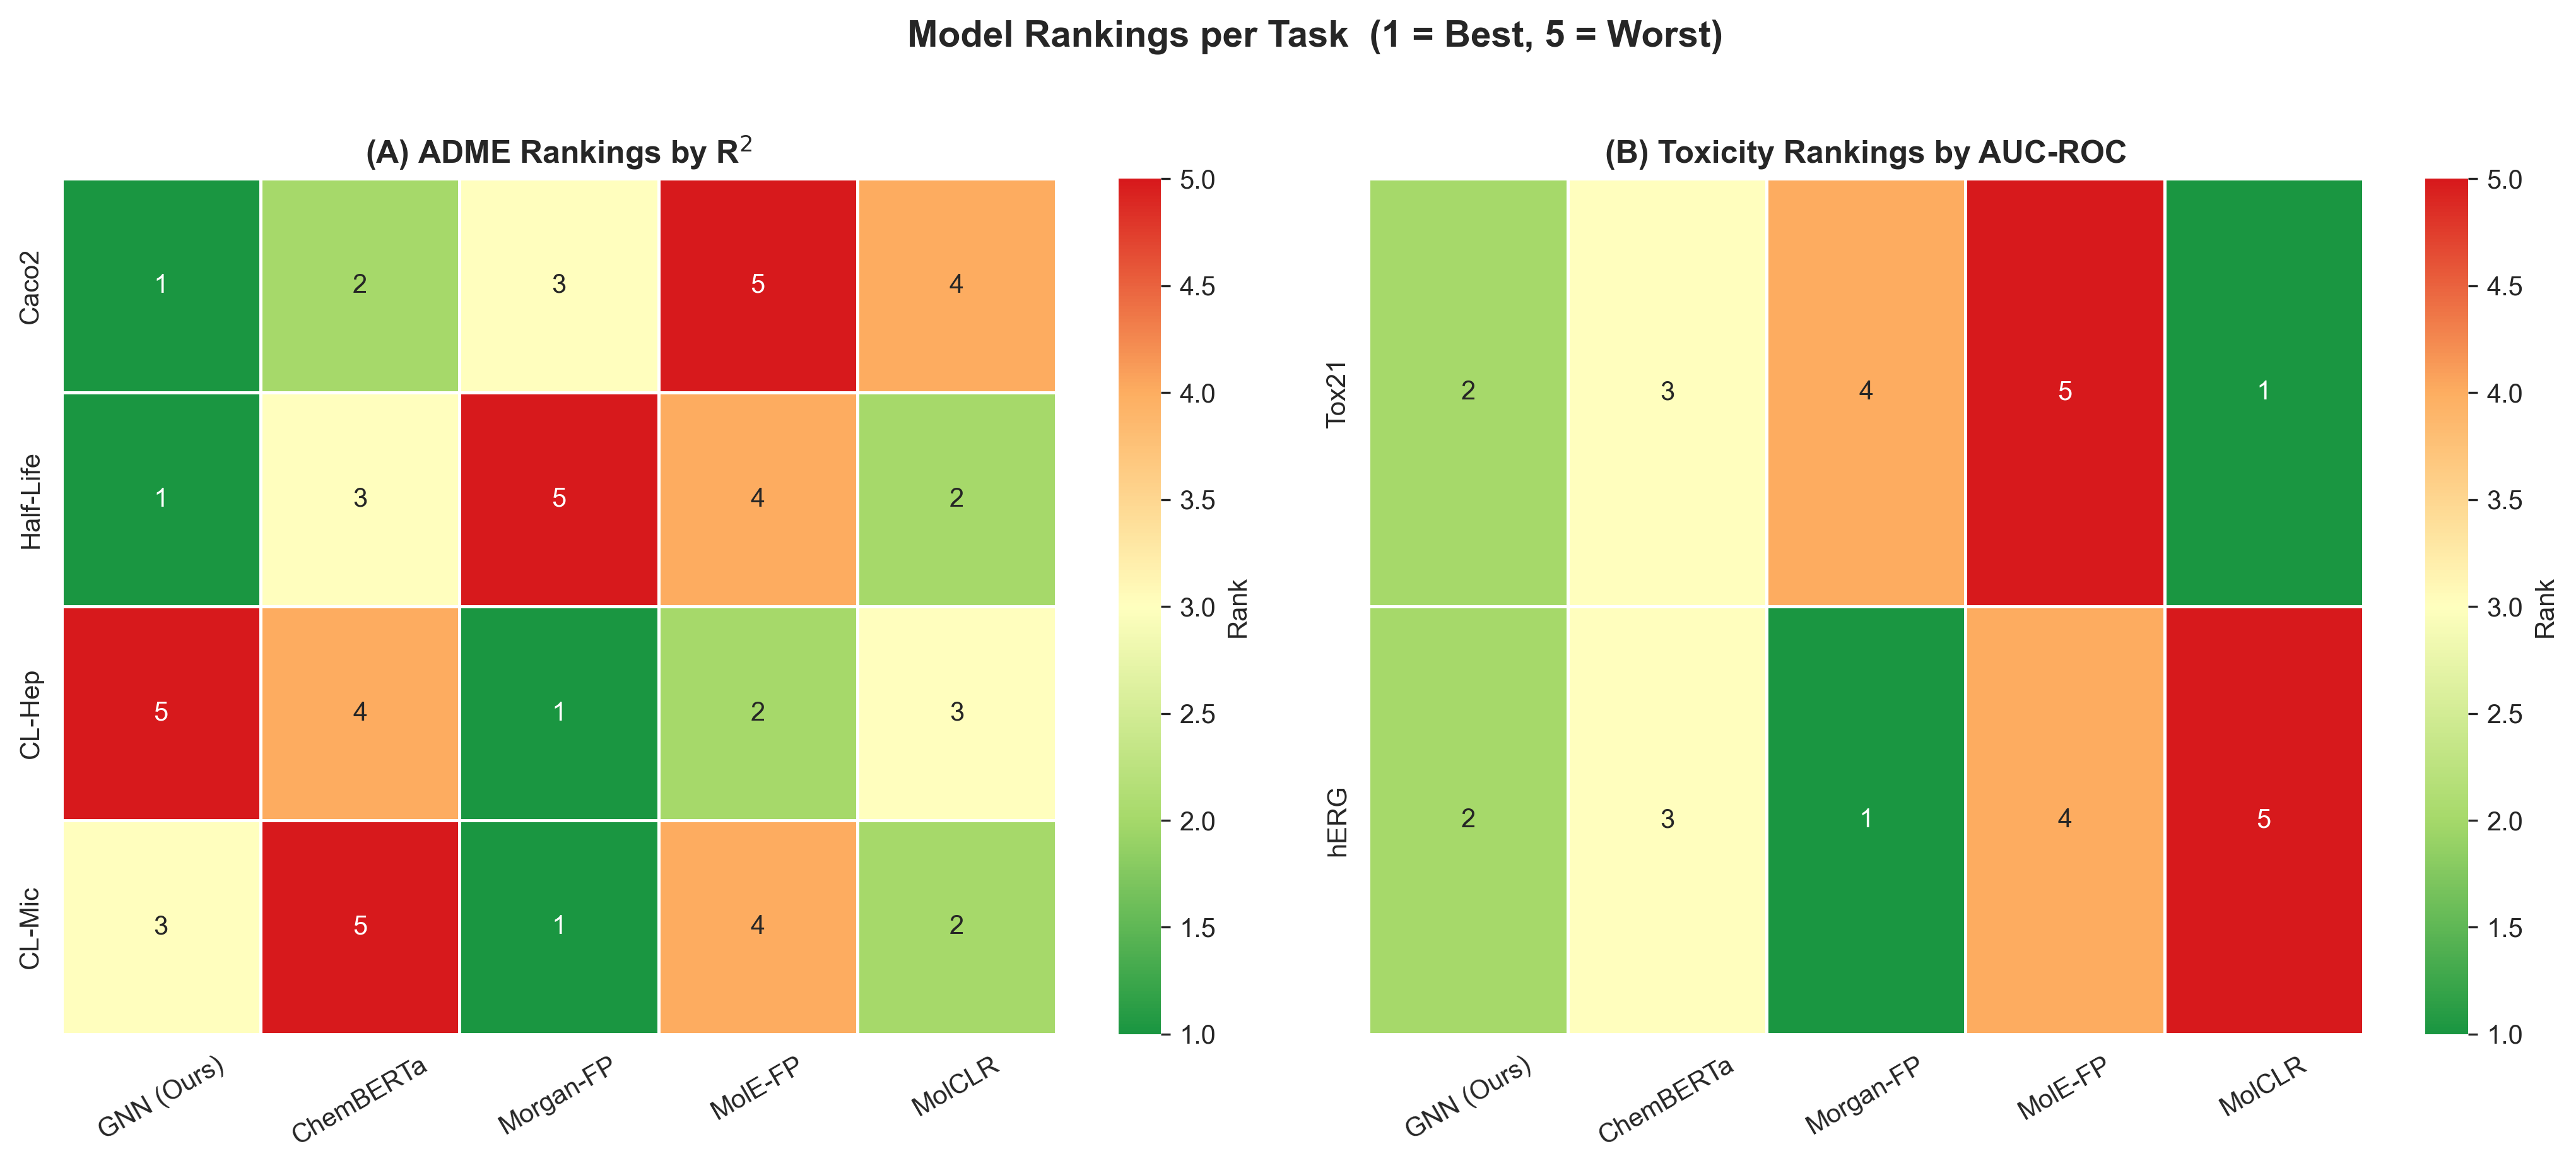
\includegraphics[width=\columnwidth,height=0.42\textheight,keepaspectratio]{foundation_ranking.png}
 \caption{Task-dependent performance of different model families across ADMET endpoints. Green indicates better performance within each task.}
 \label{fig:foundation_ranking}
\end{figure}

\begin{table*}[!t]
\centering
\caption{Fair model-family comparison across ADMET endpoints, reported as the \textbf{median over ten seeds} of each family's validation-selected configuration. Every family receives a matched 50-trial, validation-based tuning budget (GNN: random search over the architecture and training-hyperparameter space; pretrained and fingerprint models: search over the MLP prediction head on frozen features), and each selected configuration is evaluated once on an identical scaffold-split test set; no test information is used for any selection. R$^2$ (regression) and AUC-ROC (classification); higher is better. Bold marks the highest median per endpoint, but the leading families are typically separated by less than the across-seed range, so these should be read as evidence that no family dominates rather than as significant wins. Per-seed ranges are reported in the Supplementary Material. R$^2$ is scale-invariant across the different target preprocessings; a negative R$^2$ indicates performance worse than the constant predictor equal to the mean of the observed test targets, and on the weakly-learnable clearance and half-life endpoints some validation-selected configurations diverge on a minority of seeds (individual per-seed R$^2$ reaching strongly negative values, reported raw without any capping), which is why medians rather than means are reported.}
\label{tab:model_comparison}
\small
\begin{tabular}{llccccc}
\toprule
\textbf{Task} & \textbf{Metric} & \textbf{GNN} & \textbf{ChemBERTa} & \textbf{Morgan-FP} & \textbf{MolE-FP} & \textbf{MolCLR} \\
\midrule
\multicolumn{7}{l}{\emph{Group 1: Structure-driven tasks}} \\
\midrule
hERG & AUC $\uparrow$ & 0.754 & 0.747 & \textbf{0.767} & 0.735 & 0.657 \\
Caco-2 & R$^2$ $\uparrow$ & \textbf{0.482} & 0.413 & 0.322 & 0.127 & 0.232 \\
\midrule
\multicolumn{7}{l}{\emph{Group 2: Partially structure-driven tasks}} \\
\midrule
Tox21 (NR-AR) & AUC $\uparrow$ & 0.718 & 0.714 & 0.706 & 0.698 & \textbf{0.722} \\
Clearance Mic. & R$^2$ $\uparrow$ & 0.093 & $-$0.010 & \textbf{0.169} & 0.056 & 0.125 \\
\midrule
\multicolumn{7}{l}{\emph{Group 3: Tasks weakly learnable from structure alone}} \\
\midrule
Half-Life & R$^2$ $\uparrow$ & \textbf{$-$0.010} & $-$1.918 & $-$6.341 & $-$3.776 & $-$0.672 \\
Clearance Hep. & R$^2$ $\uparrow$ & $-$0.373 & $-$0.224 & \textbf{$-$0.017} & $-$0.106 & $-$0.113 \\
\bottomrule
\end{tabular}
\end{table*}

\paragraph{Group 1: Structure-driven tasks.}
On hERG and Caco-2 the models reach their highest scores, but no single family is clearly best. On hERG the leading families lie within $0.03$ AUC of one another (Morgan-FP highest at $0.77$, with the GNN and ChemBERTa at $0.75$), a spread smaller than the across-seed range, so we do not read any as a significant winner. On Caco-2 the GNN attains the highest median R$^2$ ($0.48$), but the controlled ablation below shows this advantage comes entirely from the auxiliary physicochemical descriptors: without them the graph model collapses. These endpoints have relatively strong structure--activity relationships---hERG channel blockade tracks specific pharmacophoric motifs, and intestinal permeability tracks molecular size, lipophilicity, and hydrogen-bond capacity---which SMILES transformers and fingerprints capture as well as a graph model.

\paragraph{Group 2: Partially structure-driven tasks.}
On Tox21 and Microsomal clearance predictive power is moderate and, again, closely matched. On Tox21 all families lie between AUC $0.70$ and $0.72$ (MolCLR highest at $0.722$, GNN $0.718$); on Microsomal clearance Morgan-FP gives the highest median R$^2$ ($0.17$), ahead of MolCLR ($0.13$) and the GNN ($0.09$). Structure is partially informative here, but no model family dominates.

\paragraph{Group 3: Tasks weakly learnable from structure alone.}
On Half-Life and Hepatocyte clearance all families produce near-zero or negative R$^2$. The best Half-Life median R$^2$ is only $\approx 0$ ($-0.01$, GNN), and every other family is negative---strikingly so for the fingerprint baselines, whose validation-selected heads overfit these tiny scaffold-split training sets and collapse to large negative test R$^2$ (Morgan-FP $-6.3$, MolE-FP $-3.8$). On Hepatocyte clearance the best median is Morgan-FP ($-0.02$); the GNN's validation-selected configuration is unstable on this endpoint and posts a strongly negative median R$^2$ ($-0.37$), with individual seeds reaching strongly negative raw R$^2$ values (Table~\ref{tab:multiseed}). These results indicate that, for the structure-only representations evaluated here under scaffold splitting, molecular structure alone does not support robust prediction of these pharmacokinetic endpoints, which depend on enzyme kinetics, transporter activity, protein binding, and individual patient variability~\cite{obach1999prediction}. The similarly weak performance across simple and complex models points to a limitation in the information content of structure-only representations rather than the choice of learning algorithm.

\subsection{Model Performance Across Tasks}
\label{sec:model_performance}

Fig.~\ref{fig:foundation_comparison} compares GNN, pretrained, and fingerprint models across all tasks.

\begin{figure*}[!t]
 \centering
 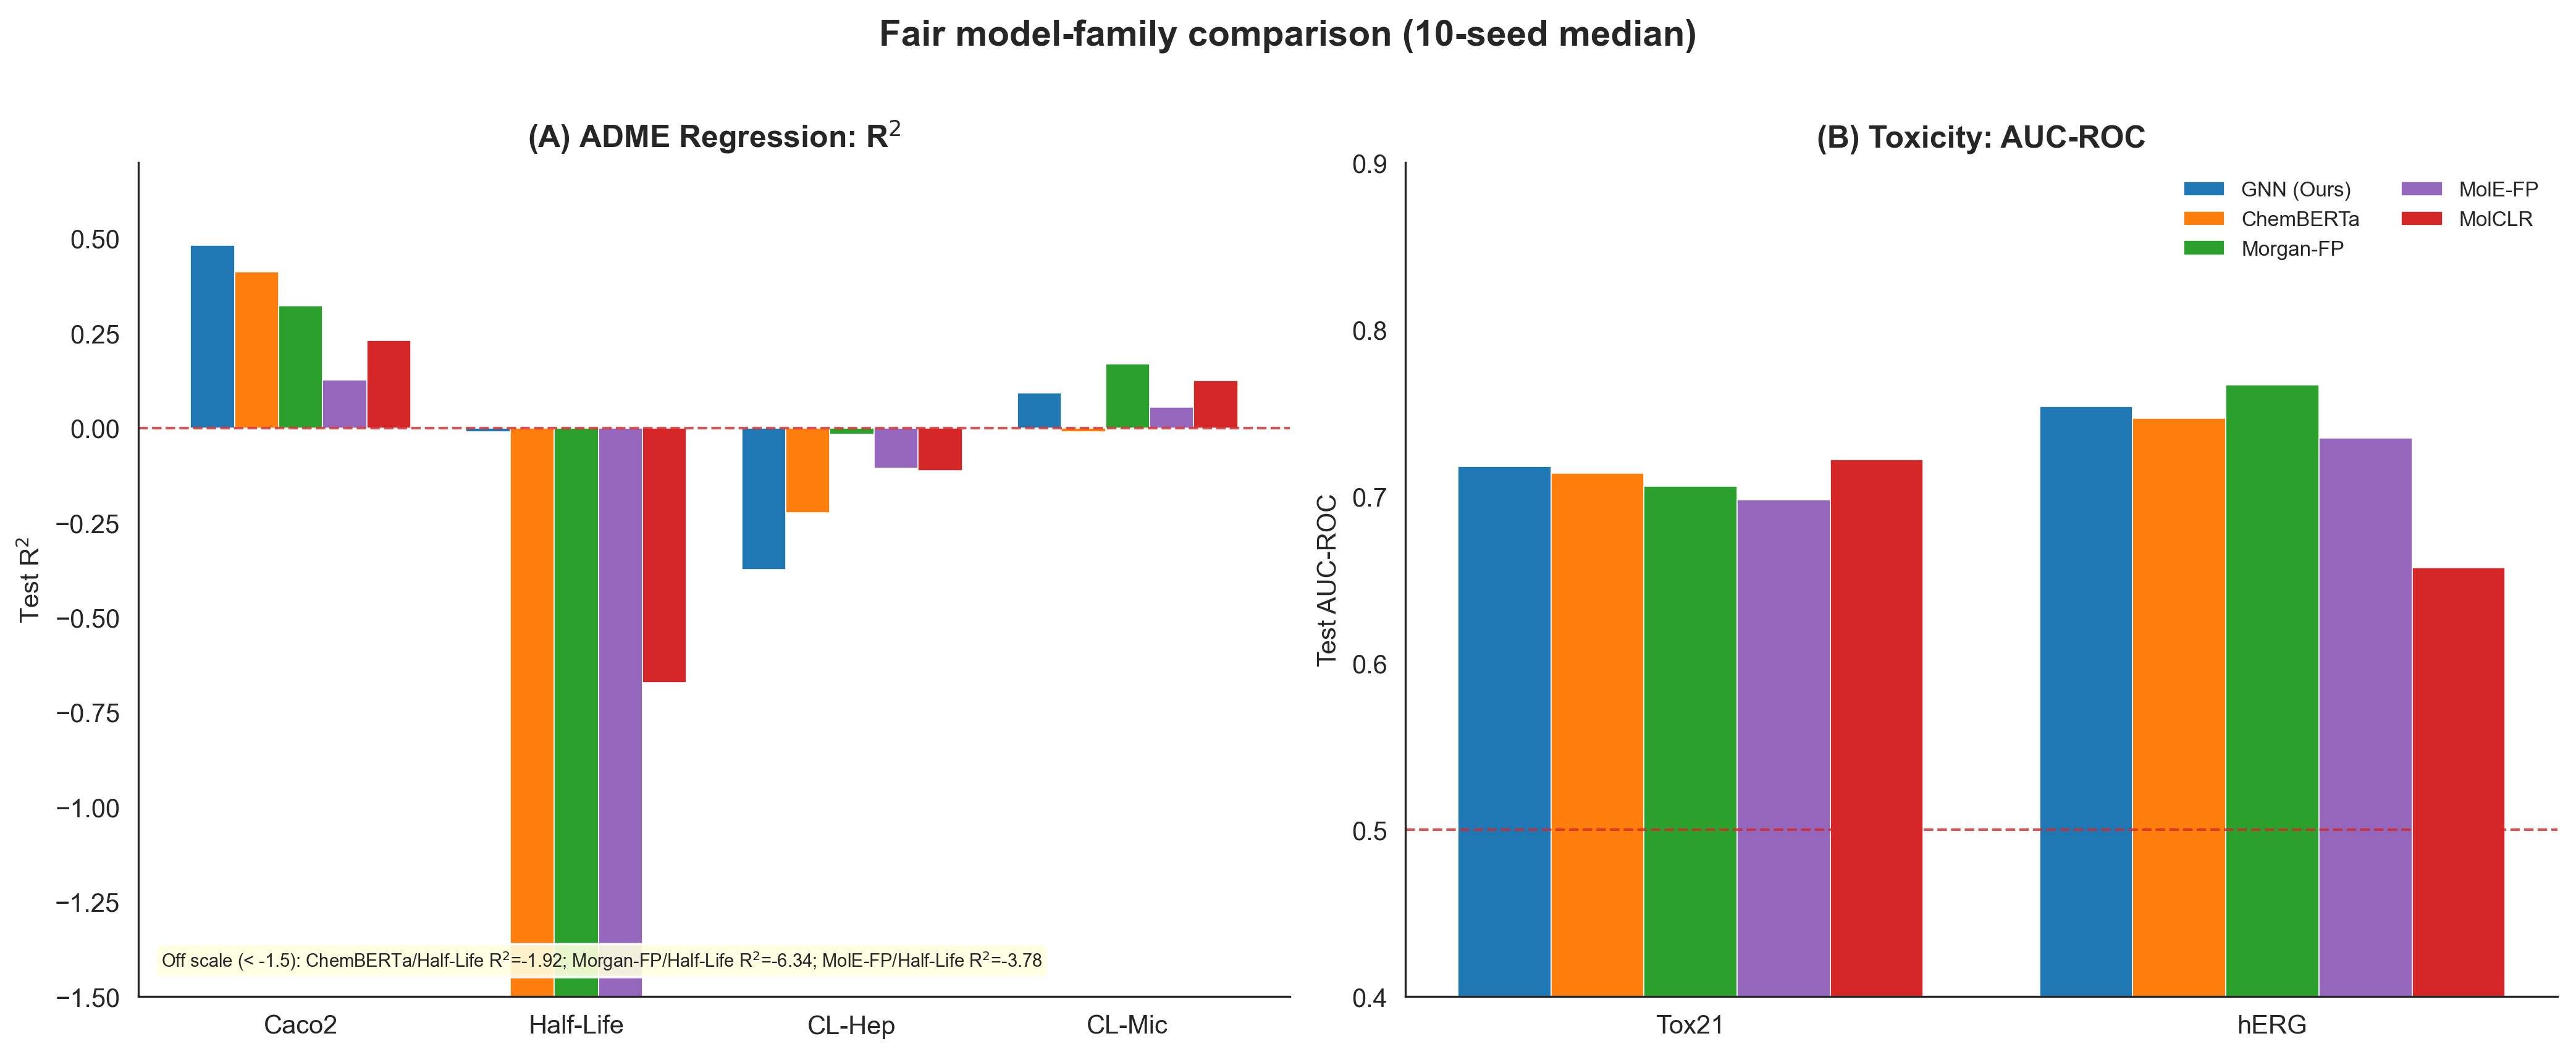
\includegraphics[width=0.85\textwidth,height=0.45\textheight,keepaspectratio]{gnn_vs_foundation_comparison.png}
 \caption{Comparison of GNN (with HPO) against pretrained and fingerprint baselines across all datasets, using the metrics reported in Table~\ref{tab:model_comparison}. (A) ADME regression R$^2$ (higher is better, dashed line at $R^2=0$), (B) toxicity AUC-ROC (dashed line at the 0.5 random baseline).}
 \label{fig:foundation_comparison}
\end{figure*}

\paragraph{The GNN's one advantage is descriptor-driven.}
The GNN alone receives auxiliary physicochemical descriptors---a compact set of 15 RDKit-computed features (7 for Caco-2), not the 200-dimensional RDKit2D block used by the RDKit2D+MLP baseline---that the frozen baselines do not. A controlled ablation (each endpoint's validation-selected configuration retrained with and without the descriptors, median over ten seeds) shows this input is decisive precisely on the one endpoint where the GNN leads: on Caco-2 the median test R$^2$ falls from $0.45$ with descriptors to $-0.51$ without them ($\Delta = +0.97$), so the GNN's Caco-2 advantage is attributable to the descriptors rather than to graph message passing. On the two toxicity endpoints the descriptors add essentially nothing (hERG $\Delta \approx +0.00$, Tox21 $\Delta \approx +0.01$): the graph model alone (hERG $\approx 0.76$) already performs at the level of the fingerprint and pretrained baselines. On the weakly-learnable clearance and half-life endpoints the effect is small or mixed (Half-Life $\Delta \approx +0.02$; Hepatocyte clearance $\Delta \approx -0.31$, both models near or below zero). Once tuning and inputs are matched, graph message passing itself confers no consistent advantage.

\paragraph{Comparable performance on permeability.}
On Caco-2, the GNN attains the highest median R$^2$ ($0.48$), ahead of a tuned ChemBERTa ($0.41$) and Morgan-FP ($0.32$), with low across-seed variance (Table~\ref{tab:multiseed}); as the ablation above shows, this margin comes from the auxiliary descriptors rather than the graph representation.

\paragraph{Limited performance on clearance and half-life.}
On Hepatocyte clearance, no model achieves meaningful predictive power (all R$^2$ near or below zero); the best median is Morgan-FP ($-$0.02), while the GNN's validation-selected configuration is unstable and falls to $-$0.37. Frozen representations are less extreme than end-to-end GNN training here (a tuned ChemBERTa R$^2$ = $-$0.22), indicating they can serve as regularized baselines rather than that pretrained models are superior for clearance. The same weak signal persists on Half-Life and Microsomal clearance. For practitioners, this suggests a diagnostic approach: if a task-specific GNN yields negative R$^2$ or near-random AUC on a scaffold-split test set, the endpoint may not be predictable from structure alone, and frozen encoders can be included as regularized baselines.

\subsection{Backbone Selection}
\label{sec:arch_selection}

A preliminary architecture screening was performed across eight graph neural network variants to select a backbone for the main benchmark, with each architecture evaluated at its best of five validation-selected configurations under the same scaffold-split pipeline. No single architecture dominated: ranked by \emph{validation} performance (the only leak-free selection signal), the average regression rank spans a narrow band ($3.0$--$6.0$ across eight backbones) and per-dataset validation differences are small (e.g., Caco-2 validation R$^2 = 0.51$--$0.63$, Tox21 AUC $= 0.78$--$0.85$, hERG AUC $= 0.90$--$0.92$), while on the weakly-learnable clearance and half-life endpoints every architecture is unstable (Supplementary Tables~S1 and~S2). This validation ordering is a poor predictor of test performance---several validation-competitive backbones post negative mean test R$^2$---reinforcing that predictability is endpoint-driven rather than architecture-driven. Because no backbone is meaningfully better on validation, we adopted GraphConv as a single representative message-passing backbone; it is mid-ranked on validation (regression validation rank $4.25$ of $8$) and is not a test-maximizing choice (its mean test R$^2$ is in fact among the lowest), and because selection used validation metrics only, the main-benchmark test evaluation remains unbiased. Full per-architecture results for both the classification and regression endpoints (all eight backbones, evaluated under the same scaffold-split pipeline) are provided in the supplementary material (Tables~S1 and~S2, Figs.~S1 and~S2).

\subsection{Effect of Optimization}
\label{sec:optimization}

The HPO-algorithm comparison across all endpoints is reported in the Supplementary Material. Each optimizer's configuration is selected on validation and evaluated once on the held-out test set; we then compare each optimizer to Random Search by the paired difference across the six datasets. No metaheuristic consistently outperforms Random Search: the paired 95\% bootstrap confidence intervals span zero for every optimizer. We deliberately do not name a single ``best'' optimizer per dataset, since such per-dataset winners are not stable across seeds and must not be chosen using test data.

The paired per-endpoint differences between each optimizer and Random Search across the six datasets are summarized in Supplementary Material (Table~S3), using each endpoint's primary test metric (R$^2$ for regression, AUC-ROC for classification) oriented so that positive values favor the optimizer. None of the metaheuristics shows a consistent net improvement over Random Search: no optimizer is significant under a paired sign test (the most favorable, ABC, wins on five of six endpoints but at $p=0.22$), and every scale-free direction-normalized effect and every scale-clipped mean difference has a bootstrap 95\% confidence interval that spans zero. Only the aggressively compressed floor-$0$ sensitivity variant yields two marginal effects of opposite sign (ABC slightly positive, SA slightly negative), which do not indicate a consistent winner. This indicates that, under our 50-trial budget, optimization strategy has limited impact compared to task characteristics, and that Random Search is a strong baseline rather than one that adaptive search reliably surpasses.

The competitiveness of Random Search on regression tasks is consistent with the ``effective dimensionality'' phenomenon~\cite{bergstra2012random}: when only a subset of hyperparameters dominates performance, the probability of Random Search sampling a near-optimal configuration by chance increases. Fig.~\ref{fig:algorithm_performance} compares all algorithms across datasets on test RMSE, R$^2$, and training time, where the performance-time panel shows that Random Search and PSO reach competitive accuracy at low computational cost.

The GNN's validation-selected configuration reaches ROC-AUC $>0.7$ on both classification tasks. On hERG it achieves F1 = 0.79 (PR-AUC 0.89, MCC 0.37), with balanced performance across both classes. On Tox21 the same configuration reaches F1 = 0.44 and MCC 0.49 despite high overall accuracy, reflecting the severe class imbalance ($\approx$5\% positive rate on the scaffold-split test set). Per-class confusion matrices are shown in Supplementary Materials (Fig. S3). Because ROC-AUC and accuracy can be misleading under the severe class imbalance of Tox21, we additionally report the area under the precision-recall curve (PR-AUC) and the Matthews correlation coefficient (MCC)~\cite{chicco2020mcc} as threshold-free and threshold-dependent imbalance-aware metrics, respectively; for Tox21 ($\approx$5\% positives) we treat PR-AUC as a co-primary metric alongside ROC-AUC, since a high ROC-AUC can coexist with weak minority-class detection. Across-seed stability of these metrics is shown in Supplementary Materials (Fig. S4).

\subsection{Effect of Evaluation Protocol}
\label{sec:eval_protocol}

\paragraph{Model-family differences are small under scaffold-split evaluation.}
Table~\ref{tab:multiseed} presents multi-seed validation results for the primary evaluation metrics of the best HPO-selected configurations, reported as the median [min--max] across ten seeds. Imbalance-aware toxicity metrics (PR-AUC, MCC, F1) are summarized separately using mean $\pm$ standard deviation in the Supplementary Material to emphasize across-seed variability under class imbalance. Caco-2, Half-Life, Tox21, and hERG are relatively stable across seeds, whereas the configuration diverges on a minority of seeds for Microsomal and Hepatocyte clearance, where individual seeds reach strongly negative R$^2$. We therefore report the median, which is robust to these divergent runs. The wide ranges on the clearance endpoints are consistent with our central finding that the weakly-learnable pharmacokinetic endpoints do not support robust structure-only prediction.

\begin{table}[!t]
\centering

\caption{Across-seed variability of the GNN's validation-selected configuration (the GNN column of Table~\ref{tab:model_comparison}), evaluated with the GraphConv backbone as the median [min--max] over ten seeds $[42, 123, 456, 789, 1011, 2022, 3033, 7, 99, 2718]$. The median is used because the configuration diverges on a minority of seeds for Microsomal and Hepatocyte clearance (individual seeds reaching strongly negative R$^2$); the ranges quantify this instability. Regression is shown as RMSE here to complement the scale-invariant R$^2$ of Table~\ref{tab:model_comparison}.}
\label{tab:multiseed}
\small
\begin{tabular}{lccc}
\textbf{Dataset} & \textbf{Task} & \textbf{Metric} & \textbf{Median [min--max]} \\
\midrule
Caco2 & Regr. & RMSE & 0.0027 [0.0025--0.0035] \\
Half\_Life & Regr. & RMSE & 21.80 [18.40--22.86] \\
Clear.\_Hep. & Regr. & RMSE & 56.22 [46.53--977.95] \\
Clear.\_Mic. & Regr. & RMSE & 41.03 [38.48--55.37] \\
Tox21 & Class. & AUC & 0.718 [0.695--0.749] \\
hERG & Class. & AUC & 0.754 [0.704--0.809] \\
\bottomrule
\end{tabular}
\end{table}


\paragraph{Evaluation protocol influences model rankings.}
Scaffold-based splitting creates a structural covariate shift where the model must generalize not merely to unseen molecules, but to unseen chemical families. Under such conditions, validation performance becomes a noisier proxy for true generalization, because a configuration that fits the specific scaffolds in the validation set may not transfer to the test scaffolds. On Tox21, the pretrained encoders reach high validation AUC that does not carry over to the scaffold-split test set: ChemBERTa drops from validation AUC $\approx 0.92$ to a test median of $0.714$, and MolCLR from $\approx 0.90$ to $0.722$ (Table~\ref{tab:model_comparison}). These results demonstrate that evaluation protocol substantially influences model rankings and perceived performance. Partial fine-tuning does not change this picture: unfreezing ChemBERTa's last two transformer layers (evaluated on the same canonical split as every other model) yields test performance comparable to the frozen-feature protocol---within a few points on the classification endpoints (hERG AUC $0.770$ vs.\ $0.747$ frozen; Tox21 $0.735$ vs.\ $0.714$), positive only on Caco-2 (R$^2 = 0.39$), and near-zero or negative on the harder regression endpoints (Half-Life $-0.08$, Hepatocyte clearance $-0.25$). Fine-tuning neither rescues the difficult pharmacokinetic tasks nor overturns the frozen-feature ranking, so the frozen protocol used for the pretrained models does not understate their performance here.

The noise introduced by scaffold splitting also explains why, within the evaluated datasets and 50-trial budget, we did not observe consistent evidence that the evaluated HPO strategies outperform Random Search, seen in Supplementary Materials (Table S3): no optimizer is significant under a paired sign test, and every scale-free and scale-clipped paired confidence interval spans zero. Adaptive methods use validation performance to guide search decisions, but when that signal is noisy, they risk optimizing for the specific validation fold rather than discovering genuinely superior hyperparameters. Random Search, by contrast, does not condition on previous evaluations, making it less susceptible to sequential overfitting of a noisy validation surface.

\begin{figure*}[!t]
 \centering
 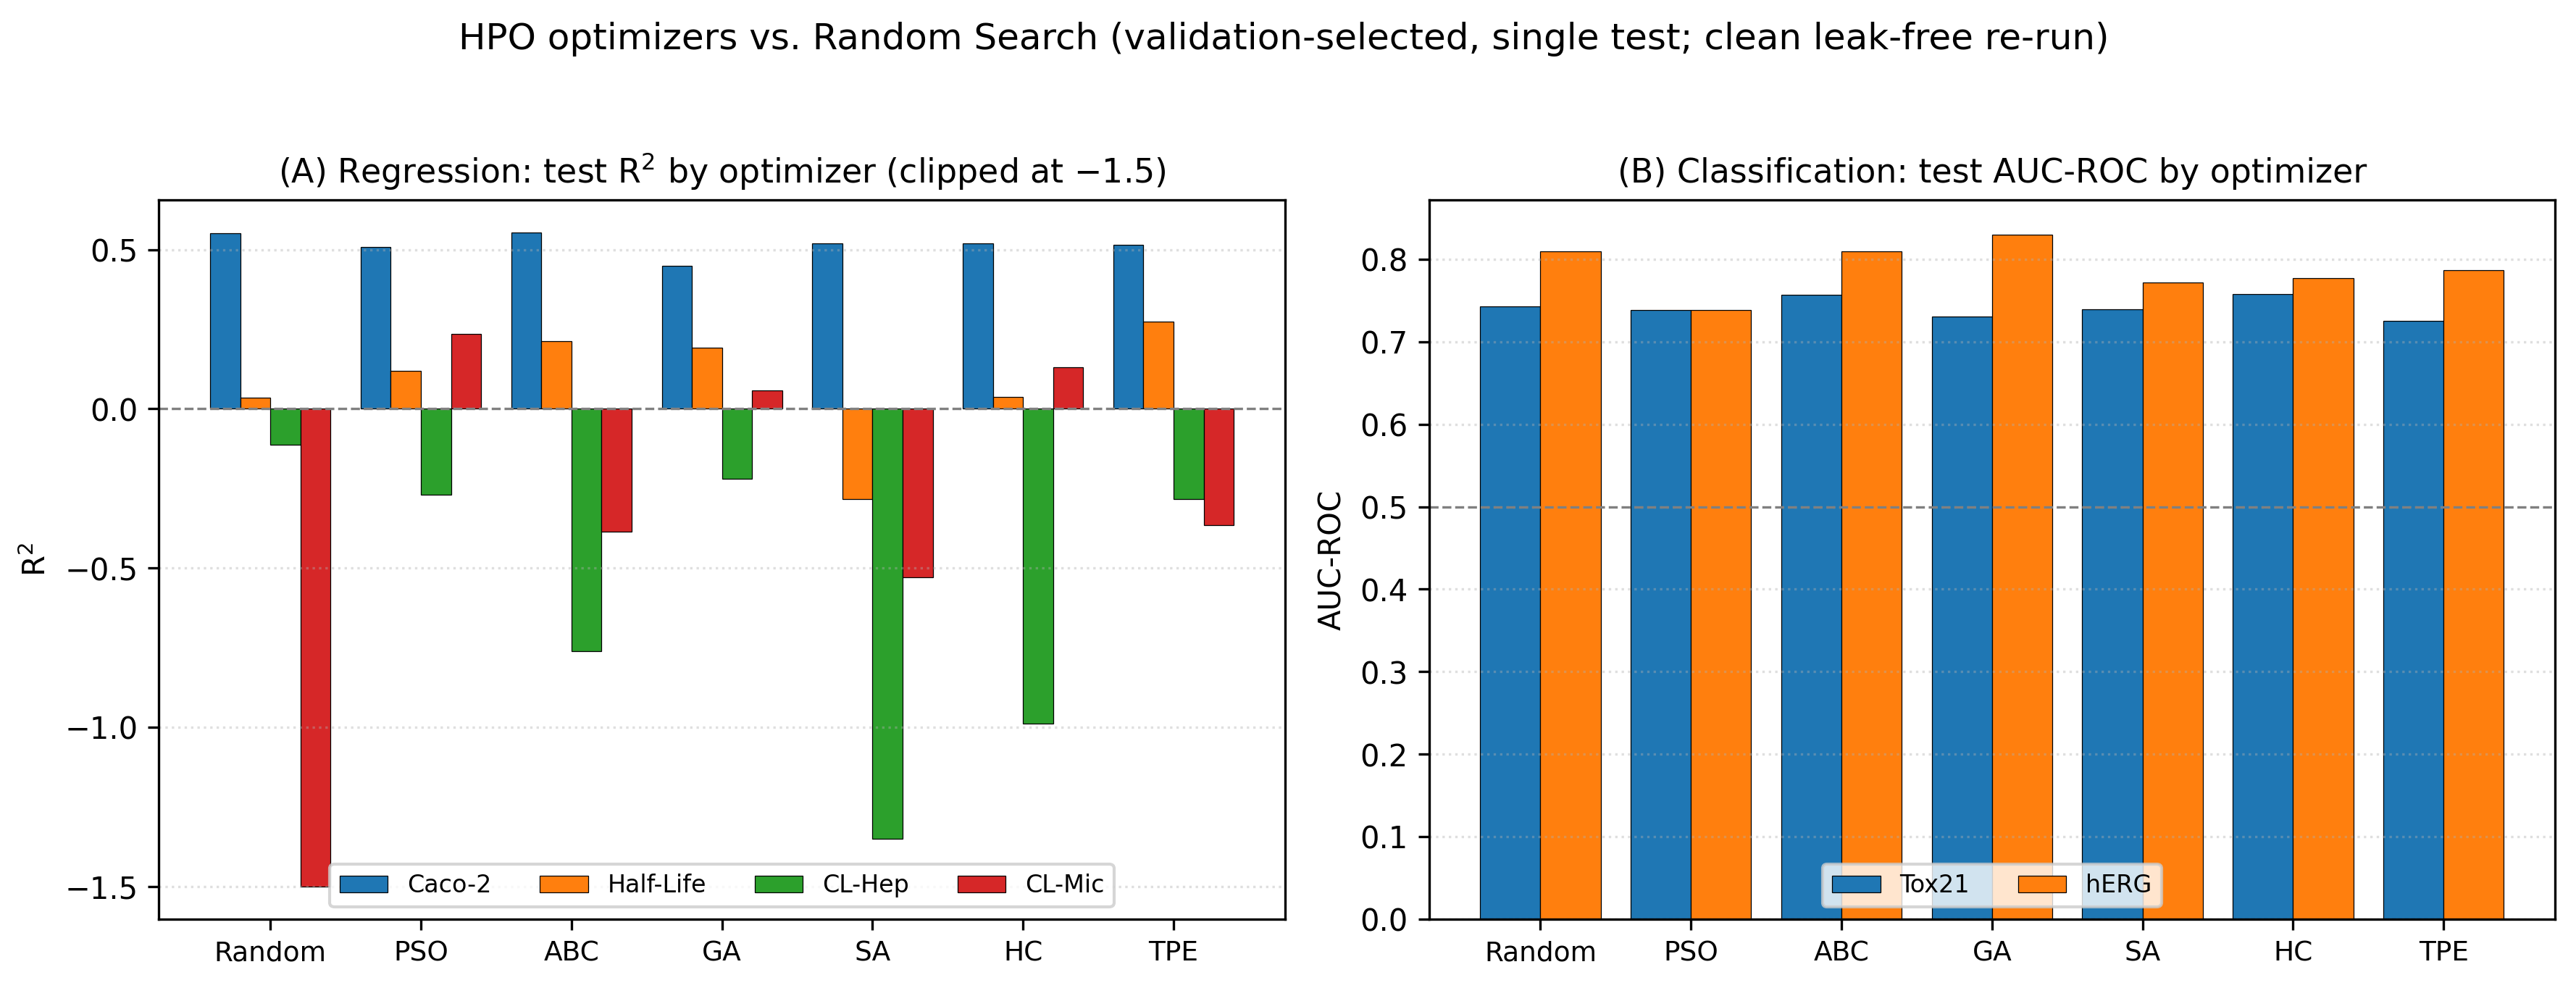
\includegraphics[width=0.80\textwidth,height=0.37\textheight,keepaspectratio]{01_algorithm_performance.png}
 \caption{HPO optimizer comparison (clean, leak-free re-run): each optimizer's \emph{validation-selected} configuration evaluated once on test. (A) Regression test R$^2$ per optimizer across the four ADME endpoints (clipped at $-1.5$ for readability; dashed line at $R^2=0$); (B) classification test AUC-ROC across the two toxicity endpoints (dashed line at the $0.5$ random baseline). No optimizer is consistently ahead of Random Search; see Supplementary Table S3 for the paired statistics.}
 \label{fig:algorithm_performance}
\end{figure*}

\section{Discussion}
\label{sec:discussion}

Predictive performance varied widely across the six endpoints, from R$^2$ = 0.48 on Caco-2 permeability to a strongly negative median R$^2$ ($-$0.37) on hepatocyte clearance, confirming that ADMET prediction is strongly endpoint-dependent. Model rankings were not consistent across datasets: architectures that performed well on permeability or toxicity did not necessarily transfer to clearance or half-life prediction. This indicates that ADMET modeling should not be treated as a single homogeneous prediction problem, because each endpoint reflects a different combination of physicochemical, biological, and experimental factors that determines how much predictive signal can be extracted from molecular structure alone.

For endpoints such as Caco-2 permeability and hERG cardiotoxicity, the models reach their highest scores, suggesting that molecular topology and local chemical environments carry useful predictive signal. This signal is captured comparably by atom-level graph message passing (our GNN uses atom features and molecular connectivity, without explicit bond features), by SMILES transformers, and by simple substructural fingerprints---no representation is distinctly better---and on Caco-2 the graph model's apparent edge derives from auxiliary physicochemical descriptors rather than from message passing itself.

In contrast, Half-Life and Hepatocyte clearance depend on biological and experimental factors not encoded in molecular structure alone, including enzyme-mediated metabolism, transporter interactions, tissue distribution, and plasma protein binding~\cite{li2019dmpk,lai2022dmpk,bohnert2013proteinbinding}. The poor performance across model families is therefore better explained by limitations of structure-only representations than by architecture: increasing model complexity did not compensate for the lack of biological context.

The classification results further demonstrate the importance of endpoint-specific evaluation. Although both toxicity tasks are classification problems, they differ substantially in class balance and biological mechanism. The Tox21 NR-AR task is highly imbalanced ($\approx$4.2\% positive rate in the full corpus, $\approx$4.9\% on the scaffold-split test set), which can bias standard training objectives toward the majority class~\cite{he2009imbalanced}. This makes ROC-AUC more appropriate than accuracy for comparing classifiers, but high AUC values should be interpreted carefully when the positive class is rare; for this reason we treat PR-AUC as a co-primary metric for Tox21. Future work should evaluate further metrics such as sensitivity, specificity, and calibration error, particularly for safety-related endpoints where false negatives are costly.

The scaffold-split protocol provides a stricter evaluation setting than random splitting by assigning compounds with the same core scaffold to the same partition, reducing the risk that models exploit close structural analogues. The observed performance drops highlight the difficulty of generalizing beyond familiar chemotypes, a central challenge in practical drug discovery.

The comparison between GNNs, fingerprints, and pretrained models suggests that no single representation is uniformly optimal. The frozen pretrained encoders evaluated here can provide useful molecular embeddings, but their performance depends on the alignment between the pretraining objective, the molecular representation, and the downstream endpoint. Classical fingerprint-based models remain competitive for some endpoints, especially when the dataset is small or the target is strongly associated with known physicochemical properties. These results support endpoint-specific model selection rather than the use of a single architecture across all ADMET tasks.

The HPO results also suggest that optimization should be interpreted cautiously. None of the evaluated metaheuristics consistently improved on Random Search: no optimizer is significant under a paired sign test, and their scale-free and scale-clipped paired 95\% confidence intervals span zero. Where individual algorithms win on a particular dataset, the advantage is small and does not transfer across datasets. For small and noisy ADMET datasets, validation performance may be unstable, and aggressive optimization can overfit to the validation split. This reinforces the need for repeated runs, consistent evaluation protocols, and transparent reporting of variance across seeds. In practice, simple optimization strategies may be sufficient for some endpoints, while more expensive search methods should be justified by consistent improvements across independent runs. Therefore, ADMET predictors should be interpreted as endpoint-specific decision-support tools: structure-only models may support hERG and Caco-2 screening, but clearance and half-life predictions require additional biological context.

This study has several limitations. First, the benchmark focuses on six TDC ADMET endpoints, which cover important but not exhaustive aspects of drug safety and pharmacokinetics. Second, the pretrained encoders (ChemBERTa, MolCLR) are evaluated primarily in a frozen feature-extraction setting; a partial fine-tuning check across all six endpoints (last two transformer layers, same canonical split) performed comparably to the frozen ChemBERTa baseline---neither consistently better nor worse (Section~\ref{sec:eval_protocol})---so the frozen setting does not understate its performance here, though a broader study across additional pretrained encoders remains future work. The encoders are also treated as representative rather than exhaustive examples. Third, all model families operate on structure-only inputs, so biological and experimental covariates (assay conditions, metabolizing enzymes, transporter and protein-binding measurements) are not included; the end-to-end GNN also receives structure-derived physicochemical descriptors that the frozen encoders and fingerprint baselines do not, so the model-family comparison is not strictly input-matched. Fourth, scaffold splitting is a more realistic protocol than random splitting but is still a retrospective benchmark, not a full prospective validation. Fifth, the datasets are small and, for the toxicity tasks, class-imbalanced, which increases variance across splits. Finally, the HPO comparison is limited to a 50-trial budget, however, a larger budget could alter the relative standing of the metaheuristics. Accordingly, our conclusions apply within the evaluated datasets, model families, scaffold-split protocol, and frozen/pretrained setup.

Future extensions include multimodal representations incorporating biological context and uncertainty-aware evaluation.


\section{Conclusion}
\label{sec:conclusion}

We benchmarked graph neural networks, frozen pretrained molecular representations, and fingerprint baselines across six TDC ADMET endpoints under scaffold-split evaluation, with a matched 50-trial validation-based tuning budget per family and ten-seed evaluation. Performance varied substantially across endpoints---moderate on hERG and Caco-2, near-zero on Half-Life and Hepatocyte Clearance---but \emph{no single model family dominated}: once tuning, seeds, and the evaluation split are matched, the leading families are separated by less than the across-seed range on most endpoints, and simple Morgan fingerprints are competitive throughout. The GNN's one clear edge (Caco-2) is attributable to auxiliary physicochemical descriptors rather than to graph message passing.

Scaffold-split evaluation is critical for drawing realistic conclusions from ADMET benchmarks. Random splits can produce overly optimistic estimates by allowing structurally similar molecules into both training and test sets, whereas scaffold splitting provides a stricter assessment of generalization to unseen scaffolds. Under scaffold-split evaluation, model-family differences are small and model rankings are endpoint-dependent. We further show that no HPO algorithm consistently outperforms Random Search at a 50-trial budget, with paired 95\% confidence intervals that span zero, reinforcing that evaluation protocol strongly influences the apparent benefit of both model architecture and optimization methods.

Future work should move beyond structure-only prediction by incorporating protein targets, assay conditions, experimental metadata, and pharmacokinetic context, and should investigate uncertainty-aware evaluation protocols that better reflect prospective drug discovery.

We summarize the endpoints as three descriptive levels of learnability from molecular structure---structure-driven (hERG, Caco-2), moderately structure-driven (Tox21 NR-AR, Microsomal Clearance), and weakly structure-driven (Half-Life, Hepatocyte Clearance). These are descriptive summaries of the present six-endpoint benchmark, not validated universal thresholds. Finally, we found that two common shortcuts---selecting the hyperparameter optimizer on the test set, and reporting single best-of-many-trial runs---can substantially inflate a favored model's apparent advantage; controlling for both was necessary to reach the conclusions above. Reliable ADMET modeling therefore requires endpoint-specific model selection together with fair, leakage-controlled, seed-averaged scaffold evaluation, supporting a cautious use of molecular AI as decision support in early-stage drug discovery rather than as a universally reliable predictor.


\section*{Data and Code Availability}
All datasets used in this study are publicly available through the Therapeutics Data Commons (TDC). The source code, trained model configurations, hyperparameter-optimization logs, and experimental results are available at:
\begin{center}
\url{https://github.com/NitramVonemats/ADMET-Benchmark}
\end{center}

Multi-seed validation used the fixed seeds $[42, 123, 456, 789, 1011, 2022, 3033, 7, 99, 2718]$, and each HPO algorithm was run for 50 trials per dataset. Software dependencies and exact versions are documented in the repository, including Python~$\geq$~3.8, PyTorch~$\geq$~2.0, PyTorch Geometric, RDKit, PyTDC, NiaPy, Optuna, and Transformers.

\section*{Ethical Compliance}
This study uses only publicly available benchmark datasets from the Therapeutics Data Commons and does not involve human subjects, identifiable patient data, animal experiments, or newly collected clinical data. Therefore, institutional review board approval and informed consent were not required.

\bibliographystyle{IEEEtran}
\bibliography{refs}

\end{document}